\documentclass[hidelinks,a4paper,10pt, nofootinbib]{article}
\usepackage[width=15.5cm, left=3cm, top=2.5cm, right=2cm, left=2cm, height= 24.5cm]{geometry}
\usepackage[spanish]{babel}
\usepackage[utf8]{inputenc}
\usepackage[T1]{fontenc}
\usepackage{xspace}
\usepackage{xargs}
\usepackage{fancyhdr}
\usepackage{lastpage}
\usepackage{caratula}
\usepackage[bottom]{footmisc}
\usepackage{amssymb}
\usepackage{amsmath}
\usepackage{algorithm}
\usepackage{algpseudocode}
\usepackage{listings}
\usepackage{hyperref} % links en índice
\usepackage{tabularx} % tablas copadas

\usepackage{graphicx}
\usepackage{sidecap}
\usepackage{wrapfig}
\usepackage{caption}
\usepackage{tikz}
\usepackage{alltt}

% facilitates the creation of memory maps. Start address at the bottom, end address at the top.
% syntax: \memsection{end address}{start address}{height in lines}{text in box}
\newcommand{\memsection}[4]{
\bytefieldsetup{bitheight=#3\baselineskip}    % define the height of the memsection
\bitbox[]{10}{
\texttt{#1}     % print end address
\\ \vspace{#3\baselineskip} \vspace{-2\baselineskip} \vspace{-#3pt} % do some spacing
\texttt{#2} % print start address
}
\bitbox{16}{#4} % print box with caption
}


%%fancyhdr
\pagestyle{fancy}
\thispagestyle{fancy}
\addtolength{\headheight}{1pt}
\lhead{Organización del Computador II: TP2}
\rhead{$2º$ cuatrimestre de 2016}
\cfoot{\thepage\ / \pageref{LastPage}}
\renewcommand{\footrulewidth}{0.4pt}
\fancyfoot[LO]{\small{Freidin Gregorio, Taboh Sebastián, Romero Lucía Inés}}
%%caratula
\materia{Organización del Computador II}
\titulo{Trabajo Práctico III}
\subtitulo{System Programming}
\grupo{Grupo: El Arquitecto}

\begin{document}

\thispagestyle{empty}
\materia{Organización del Computador II}
\submateria{Segundo Cuatrimestre de 2016}
\titulo{Trabajo Práctico III}

\integrante{Freidin, Gregorio}{433/15}{gregoriofreidin@gmail.com}
\integrante{Taboh, Sebastián}{185/13}{sebi\_282@hotmail.com}
\integrante{Romero, Lucía Inés}{272/15}{luciainesromero@hotmail.com}

\maketitle
\clearpage

\tableofcontents

\clearpage


\section{GDT}
\par{La Tabla de descriptores global o GDT es la encargada de organizar el sistema de segmentación entre otras cosas. Almacena descriptores los cuales pueden ser de segmento, de TSS, de LDT o de call gate. En nuestro sistema contamos con una estructura, gdt$\_$entry, la cual completamos con descriptores de segmentos y de tss.}
\subsection{Descriptores de Segmento}
\par{
Cada descriptor de segmento nos habilita distintas secciones de la memoria. En el caso del tp, nuestro sistema usa segmentación flat, por ende cada descriptor se maneja con el mismo rango de memoria, pero lo que cambia son los atributos con los que se accede a ella.
\begin{itemize}
\item Descriptor Nulo (requerido por Intel).
\item Descriptores Nulos desde la entrada 1 hasta la 17 (requeridos por el tp).
\item Descriptor de Segmento de Código de nivel 0 (privilegios de supervisor y lectura habilitada).
\item Descriptor de Segmento de Código de nivel 3 (privilegios de usuario y lectura habilitada).
\item Descriptor de Segmento de Datos de nivel 0 (privilegios de supervisor y escritura habilitada).
\item Descriptor de Segmento de Datos de nivel 3 (privilegios de usuario y escritura habilitada).
\item Descriptor de Segmento de video 
\end{itemize}
\medskip
\par{Los descriptores previos tenían como base 0x0000, y como límite, 0x6fff, además, el bit de granularidad seteado, por ende cada uno de los segmentos referencia los primeros 1.75 GB. Excepto por el descriptor de segmento de video, el cual posee como base: 0xb800, límite: 0x0f9f y la granularidad en 0.
Todos tenían el bit de sistema en 1 y el de presente también seteado.
}
\medskip

\subsection{Descriptores de TSS}
Luego tenemos las entradas de las tareas, en las cuales profundizaremos más adelante.
\begin{itemize}
\item Descriptor de la Tarea Inicial.
\item Descriptor de la Tarea Idle.
\item De la entrada 25 hasta la 32, nos encontramos con descriptores de tss para cada una de las tareas de nuestro sistema.
\item De la entrada 33 hasta la 40, nos encontramos con descriptores de tss para cada una de las banderas de nuestro tp.
\end{itemize}


\begin{alltt}
\normalfont
		       Todos estos descriptores mantienen el siguiente formato:
		       
         \textbf{Limite:} 0x67
			   
         \textbf{Base:} Dirección de la tss
                     
         \textbf{Presente:} Seteado
                     
         \textbf{Tipo:} 0x9. Combinado con el bit de sistema en 0, tipo 9 se refiere a un descriptor de TSS.
                
         \textbf{Sistema:} 0x0
                     
         \textbf{DPL:} 0x0. Esto es ya que en nuestro sistema queremos que las tareas sólo puedan ser accedidas por
         el kernel, es decir, que no se pueda "saltar" de una tarea a otra.
			 	
         \textbf{Granularidad:} 0x0
                     
         \textbf{AVL:} 0x0
                     
         \textbf{DB:} 0x1 (32 bits)
                     
         \textbf{L:} 0x0
\end{alltt}
}

\section{Modo Protegido}
\par{Al inicio de nuestro sistema nos encontramos en modo real. Esto es consecuencia de la condición de COMPATIBILIDAD de intel. Al iniciar nuestro sistema tenemos un 8086, nuestro código es de \textbf{16 BITS}; \textbf{NO} hay protección de memoria; podemos utilizar \textbf{TODAS} las instrucciones; AX,CX,DX \textbf{NO} son de propósito general. Y además, sólo podemos direccionar 1 MB de memoria. Por esto, luego de cargar los descriptores de código y datos vamos a pasar a "modo protegido", en el cual contamos con código de 32 bits, protección a memoria, y 4 GB de memoria direccionable.
}
\par{
Para poder realizar esto tenemos que encargarnos de un par de puntos previamente:
\begin{itemize}
\item Cargar el GDTR con la dirección de la GDT (LGDTR)
\item Deshabilitamos las interrupciones \textbf{EXTERNAS} (CLI)
\item Habilitamos A20, es decir, habilitamos el acceso a direcciones de memoria superiores a 2$^{20}$.
\item Seteamos el bit PE del registro CR0. (PE: Protected Mode Enable).
\end{itemize}
Entonces, con el contexto ya armado, ejecutamos la instrucción: \textbf{JMP FAR [selector]:[offset]}. En el caso de nuestro TP, el selector sería 18$<<$3, ya que este es el descriptor de código de nivel 0; y como offset utilizamos una etiqueta la cual se encontraba inmediatamente a continuación de esta instrucción.
}

\clearpage

\section{Paginación}
\par{El sistema de Paginacion de memoria, es una sistema en el cual se organiza la memoria de a paginas con tamaño 4K. Este sistema describe una funcion de mapeo de las direcciones virtuales, obtenidas a travez del sistema de Segmentacion, a direcciones fisicas de memoria. Agregando de paso, nuevos niveles de privilegio, como Supervisor o User, o en que direcciones se puede leer y escribir.}
\par{En este sistema optamos por implementar un sistema de paginacion en dos niveles. Esto significa que, para implementar el mapeo de memoria virtual a fisica se utilizan los siguientes elementos: }
\begin{itemize}
	\item {\bfseries CR3: }
	\par{ En el registro de Control CR3, se va a tener guardado la direccion del Directorio de Paginas que esta actuando actualmente, en un sistema se pueden tener mucho mapeos diferentes, por lo que simplemente para cambiar el esquema de Paginación solo se tiene que remplazar el valor del CR3 por la direccion del Directorio de Paginas deseado.}
	\item {\bfseries Directorio de Páginas: }
	\par{Esta estructura consiste en un arreglo de 1024 entradas, en las cuales cada PD\_entry (entrada del Directorio de paginas) los primeros 20 bits son el prefijo de la direccion en la cual esta ubicada la Tabla de paginas correspondiente  a dicha entrada, como estan alineadas a 4K cada direccion, los ultimos 12 bits de esta direccion se asumen que son 0. Y dentro de cada PD\_entry se utilizan estos bits para establecer atributos, el bit 0 para marcar Presente, el bit 1 para marcar R/W, y el bit 2 para marcar U/S, como los principales atributos mencionados.}
	\item {\bfseries Tabla de Páginas: }
	\par{Estra estructura consiste tambien en un arreglo de 1024 entradas, en la cual cada PT\_entry los primeros 20 bits marcan la posicion donde comienza una pagina de 4K de direcciones fisicas de memoria. Nuevamente como las paginas son de 4K los últimos 12 bits de esta dirección se asumen que son 0, y dentro de la cada entrada de la PT, se utilizan para marcar atributos, los principales son los mismos que los mencionados para la PD}
\end{itemize}

\subsubsection*{Proceso de Traducion Memoria Virtual -> Memoria Fisica}
\par{ Sea D la dirección de la cual quiero obtener la direccion fisica mapeada, el proceso de obtencion es el siguiente.} 
\par {Los primero 10 bits de D (D[31:22]), van a ser utilizados como indice dentro de la Page Directory, en la cual, de la entrada obtenida  se va a sacar la direccion de la Page Table correspondiente a esta direccion.}
\par{ Los segundo 10 bits de D (D[21:12]), van a ser utilizados como indice dentro de la Page Table, en la cual de la entrada obtenida se va a sacar la direccion de la pagina de 4K en donde esta contenida la direccion fisica mapeada a D}
\par{ Por último, los ultimos 12 bits de D (D[11:0]), van a ser utilizados como Offset dentro de la pagina obtenida atravez de la Page Table. Osea la direccion final seria igual a direccion de pagina fisica 4K obtenida de PT + D[11:0]. Todo esto suponiendo que D paso todos los controles implementados en el sistema de paginación.}

\subsubsection*{Paginación De Nuestro Trabajo Práctico}
\par{En primera instancia, inicializamos el mapeo para el codigo en kernel sobre el directorio de paginas ubicado en la direccion 0x27000, donde hacemos identity mapping desde la dirección 0x00000000 a 0x0077FFFF. Asignando en la seccion de atributos de cada entrada el valor de 0x3 que significa Presente = 1, R/W = 1, y nivel Supervisor. Las demas entradas las seteamos en 0.}
\par{Luego el esquema de paginación va a cambair según la tarea que se este ejectuando, para ello inicializamos varios directorios de paginas, en el cual generamos un mapping segun corresponda a la tarea que corra actualmente, donde mantenemos el mapeo hecho para el directorio del Kernel, pero agregando paginas nivel Usuario donde la tarea se va a ejecutar.}




\newpage
\section{IDT}
\label{subsec:IDT}
\par{La IDT, Interruption Descriptor Table, se encarga de almacenar descriptores de rutinas de atención sobre interrpuciones de software, de hardware, y expeciones. Este se representa como un arreglo de maximo 2**13 entradas, de tamaño 64 bits. Estos Descriptores cargan informacion sobre, donde se hubica dicha rutina de atencion, atributos de presente, o DPL (nivel de privilegio requerido para acceder a dicha interrupcion), y el selector de segmento que se va a utilizar, en general este selector es el de Código nivel 0, ya que una interrpucion suele necesitar de accesos a nivel Kernel.}

\subsection{Rellenado de IDT}
\begin{itemize}
	\item {\bfseries Expeciones: }
	\par{Por restricciones de Intel, desde la posicion 0 hasta la 19 es donde se van a hubicar los descriptores de rutinas de atencion sobre expeciones, segun el orden que indica el manual de Intel. Estas tienen los atributos de presente en 1 y el DPL en 3, pues no queremos que ninguna tarea de nivel usuario llame a una Exepcion intencionalmente. Luego las entradas entre la 20 y la 31 estan reservadas a futuras posible exepciones, o usos que Intel les proporcione.}
	
	\item {\bfseries Interrupciones de Hardware: }
	\par{ Estas se ubican en las primeras entradas libres a partir de la 32, en particular la 32 es la interrupcion de Reloj, y la 33 la interrupcion de teclado. Ambas entradas en nuestro TP estan seteadas con el SegSel = Cod\_L0, el bit de presente en 1, y DPL = 0.}
	
	\item {\bfseries Interrpuciones de Software: }
	\par{Estas son seteadas a partir de posiciones mayores, en nuestro caso implementamos 2, en la entrada 80 y en la entrada 102. Donde la unica diferencia con las de Hardware respecto a los atributos, es que estas contienen DPL = 3, ya que queremos que puedan ser llamadas por tareas nivel usuario para ejecutar un codigo en nivel 0, esto en particular se le da el nombre de syscall.}

\end{itemize}

\subsection{Proceso de identificación de interrupción requerida}
\par{Cuando ocurre una interrpcion / exepción, el proceso basicamente es obtener el descriptor de interrupcion señalado por el Vector de Interrpciones, y de ahi saltar directamente a la rutina de atención. Ahora la forma en la que se carga dicho Vector es, para expeciones, el mismo procesador se encarga de indentificar cual es la posicion asignada a dicha interrupcion, dentro de la IDT segun Intel, y carga el vector con dicho valor.  Para interrupciones de Hardware se utiliza lo que es el PIC de interrupciones donde cuando un elemento externo solicita una interrpucion, estos estan ordenados en un orden especifico segun un handler de hardware, y este identifica cual de los aparatos fue el que la solicito, cargando de esta manera al Vector de Interrupciones. Y por último a una interrpucion de Software simplemente es el numero q le sigue a la instruccion "int" que es la utilizada para solicitar una interrpucion especifica.}

\subsection{Excepciones}
\par{ESTA ME DA IGUAL}
\subsection{Interrupción de reloj}
\subsection{Interrupción de teclado}
\par{ESTA LA HACE LUCIA}
\subsection{Int 80}
\par{ESTA LA HACE LUCIA}
\subsection{Int 102}
\par{ESTA LA HACE LUCIA}
\newpage
\section{TSS}
\newpage
\section{Scheduler}
\par{El scheduler es quien se encarga de determinar qué tarea debe ser ejecutada. Para esto contamos con dos arreglos de enteros de 8 posiciones, en el caso de nuestro TP, en el cual se almacena qué navíos/banderas pueden ejecutarse. Cada posición i representa al navío/bandera i+1, y si en dicha posición hay un 1 es que el navío/bandera continúa presente en el scheduler, y, si hay un 0, no. En el caso de nuestro TP algún navío o bandera puede cometer algún error, ya sea una excepción, en cuyo caso como vimos en la sección \ref{subsec: IDT} el handler de la interrupción se encargará de ello; o, en el caso de las banderas, estas pueden haber sido interrumpidas por el reloj antes de pasar por la int 0x50. Cualquiera sea el caso, esto conlleva a la eliminación del navío y bandera correspondiente, por esto es que contamos con los arreglos que nos determinan las posibles "siguiente tarea".}
\par{
Como bien vimos en la sección \ref{subsec: IDT}, cuando debemos eliminar un navío y su bandera, lo único que hacemos es eliminar el índice correspondiente en el scheduler con la función \textbf{inhabilitar$\_$tarea(uint error, int n)}, la cual además, nos imprime en la pantalla de estados el error que se ha cometido.
}
\par{Como el scheduler se comprende de 2 arreglos, contamos con 2 índices, una para cada uno de ellos; \textbf{current} de navíos, y \textbf{currentBanderas}. Contamos con dos funciones las cuales nos proveen el siguiente navío o bandera a ejecutarse, \textbf{sched$\_$proximo$\_$indice} y \textbf{sched$\_$proxima$\_$bandera}. A continuación mostramos un pseudocódigo que aplica a ambas funciones pero con sus respectivos \textbf{currents} y con la diferencia que \textbf{sched$\_$proxima$\_$bandera} se reinicia al llegar a 8.}

\begin{algorithm}[h!]
\caption{sched$\_$proximo$\_$indice}
\begin{algorithmic}
	\State current += 1
	\State i = 0
	\While{ tareas[current]$\%$8 == 0 and i$<$9 }
		\State current += 1
		\State i += 1
	\EndWhile
	\If{tareas[current] == 0}
	\State current = -1
	\EndIf
	\State \textbf{return} current
\end{algorithmic}
\end{algorithm}

\par{Como vimos en la sección \ref{subsec:IDT}, en nuestro TP la interrupción externa 32, la interrupción de reloj, funciona como regulador de los tiempos de las tareas. Cada navío tiene un tick de reloj para correr, si llama a una syscall, el tiempo restante de su quantum es destinado a la tarea idle. Las banderas, por su parte, también tienen un tick de reloj para ejecutarse, con la salvedad de que antes de cumplido este tiempo tienen que llamar a la syscall 0x50. En cada interrupción de reloj se determina cuál será la próxima tarea a ejecutarse.}
\par{En particular, en nuestro TP, tenemos determinado que cada 3 quantum de tareas se corren \textbf{TODAS} las banderas "disponibles", es decir, las que no han sido eliminadas del scheduler por algún tipo de error.}
\par{En resumen, las tareas/navíos se ejecutan en orden, cada 3 quantum se ejecutan las banderas que siguen en el scheduler, al cometer algún error el navío/bandera es eliminado del scheduler junto con su bandera/navío, la función proximo$\_$indice nos devuelve el índice de la tarea a ejecutarse, si es que la hay.} 
\medskip
\par{\textbf{¿Y qué sucede cuando no quedan tareas a ejecutarse?}}
\par{Sigue corriendo indefinidamente la tarea idle. Situación que efectivamente ocurre en nuestro TP.}
\newpage
\begin{wrapfigure}{r}{0.4 \textwidth}
  \begin{center}
    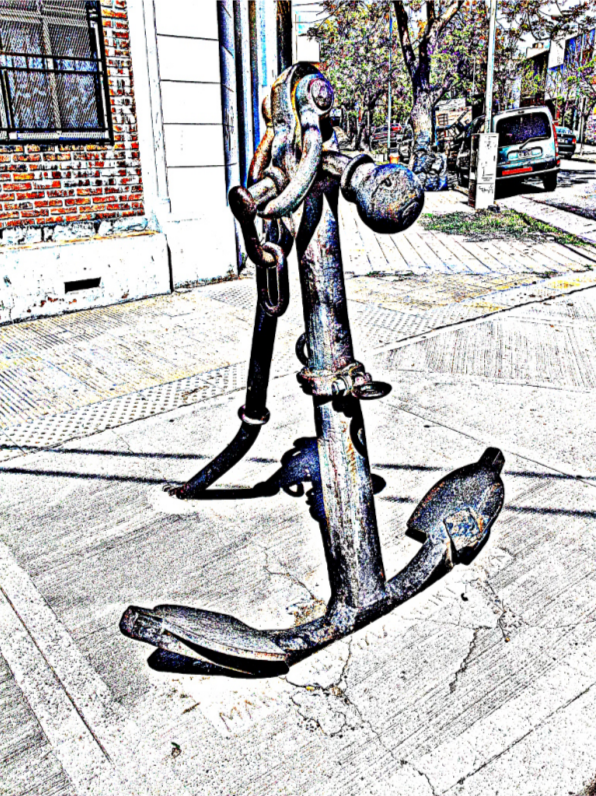
\includegraphics[scale=0.15]{imagenes/ancla.png}
  \end{center}
  \caption{Ancla}
\end{wrapfigure}
\par{
\section{Conclusión}
\bigskip
\subsection{Ancla}
}
\textcolor{white}{.}\\
\\
\bigskip
Queremos aportar a la cátedra nuestro siguiente descubrimiento: \\ 
Respondiendo al punto optativo \textbf{4.8 inciso d}, el ancla de la siguiente imagen, misma imagen que la figura 2 del enunciado del TP; se encuentra en la esquina de la intersección de las calles Pedernera y Tte. Cnel. Casimiro Recuero en el barrio porteño de Flores.

\bigskip
\bigskip
\bigskip
\bigskip
\bigskip
\subsection{Ejercicio 4.8}
\par{
Luego de implementar lo descrito en este informe, sumado a ciertas funciones para imprimir en pantalla, creemos que nuestro sistema operativo cumple con lo establecido en el TP. Sin ir más lejos nos sentimos preparados y ansiosos por consagrarnos victoriosos en el evento de "Guerra de Tareas", ya que un navío letal está siendo diseñado para dicho propósito.}

\end{document}
